% !TEX encoding = UTF-8 Unicode
\documentclass[12pt, oneside]{article}
\usepackage{geometry}
\geometry{letterpaper}
\usepackage{graphicx}
\usepackage{amssymb}
\usepackage[utf8]{inputenc}
\usepackage[francais]{babel}
\usepackage{fullpage}
\usepackage[]{algorithm2e}
\usepackage{placeins}
\usepackage{hyperref}
\hypersetup{
    colorlinks,
    citecolor=black,
    filecolor=black,
    linkcolor=blue,
    urlcolor=blue
}
\hypersetup{linktocpage}
\title{{\normalsize{INFO-F-203}}\\Projet: Les bons comptes font les bons amis}
\author{Grigore \textsc{Antoniuc} \and Pavlo \textsc{Polinetskyi}}
%\date{19/12/2016}

\SetKwProg{Fn}{Function}{}{}
\SetKwProg{Al}{Algorithm}{}{}
\begin{document}
\maketitle
\tableofcontents
\addcontentsline{toc}{section}{}
\newpage
\section{Introduction}
Ce rapport accompagne le projet d'Algorithmique de deuxième année, reposant sur la manipulation de graphes. 

L'énoncé laissant le choix du langange entre $Java$ ou $Python$, ce projet est codé en $Python 3$.   
\subsection{Le problème}
Le sujet du projet met l'étudiant dans la peau d'un informaticien devant créer un programme mobile censé gèrer les dettes entre groupes d'amis. 

Un groupe d'amis est représenté sous la forme d'un graphe dirigé lu à partir d'un fichier, dans lequel les noeuds représentent les individus et les arêtes représentent les dettes entre ceux-ci.

%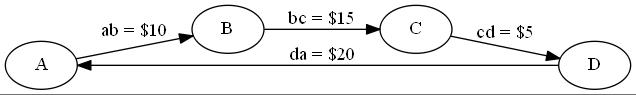
\includegraphics{2_1_0}
\subsection{Objectifs}
L'énoncé du projet demande d'implémenter plusieurs algorithmes dont nous avons choisi les suivants.
\\
\begin{itemize}
\item La simplification de dettes
\item L'identification des communautés
\item L'identification des hubs sociaux
\end{itemize}
\newpage
\section{Simplification de dettes}

\subsection{Description}
Cet algorithme reçoit en paramètre un graphe et renvoie ce même graphe, mais présentant une simplification des dettes.
\subsection{Implémentation}
\subsubsection{Explication}
La simplification du graphe est basée sur le principe que tout cycle de dettes peut être simplifié.Cela est fait en prenant la plus petite dette presente dans le cycle, et en la soustrayant de toutes les dettes du cycle. Ainsi, il est garanti qu'une dette soit reduite à 0.\\

L'algorithme fonctionne en trouvant toutes les composantes fortement connexes à l'aide de l´algorithme de Tarjan et en appliquant l'algorithme de Johnson sur celles-ci afin de trouver tous les cycles elementaires du graphe.

La derniere étape consiste dans le fait de parcourir tous les cycles, en soustrayant la dette minimale contenue dans ceux-ci.\\\\
Complexité: $O((n + e)(c + 1))$, ou $n$ est le nombre de noeuds, $e$ est le nombre d'arcs et $c$ le nombre de cycles du graphe.

\FloatBarrier
\subsection{Exemple}
\begin{figure}[!h]
    %\textbf{Your title}\par\medskip
    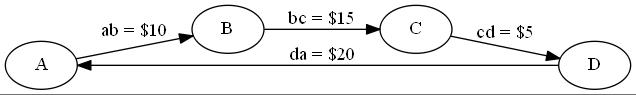
\includegraphics[trim=3 3 3 3,clip]{2_1_0}
    \caption{Supposons les relations de dettes ci-dessus}
\end{figure}

\begin{figure}[!h]
    %\textbf{Your title}\par\medskip
    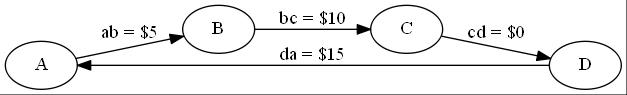
\includegraphics[trim=3 3 3 3,clip]{2_1_Simplified}
    \caption{Tel est l'état du graphe après simplification}
\end{figure}

\newpage
\subsubsection{Pseudocode}
\begin{algorithm}[!h]
\Al{Tarjan}{
  \KwResult{List of Strongly Connected Components}
	\bigskip
   \Fn{find\_sccs}{
    \KwData{allnodes, removednodes}
   \For{each node in allnodes}{
     \If{node not in removed and node not treated}{
       explore(node)
    }
   }
   }
   \bigskip
   \Fn{explore}{
    \KwData{node}
   	node.index = index
   	node.lowestbackedge = index
	node.min = index   	
   	stack.push(node)
   	
   	\For{edge in node}{
   	 \If{edge not in removed and edge not treated}{
       explore(edge)
       node.min = min(node.min, edge.lowestbackedge)
     }
   	}
   	\If{node.min $<$ node.lowestbackedge}{
   	 node.lowestbackedge = node.min
   	}
   	\Else{
   		We have found a strongly connected component\\
   		Pop nodes from the stack until we reach this node and add them to list of sccs.\\ 
   	}
   }
}
\end{algorithm}

\begin{algorithm}[!h]
\Al{Cycles\_Johnson}{
  \KwResult{List of Cycles}
	\bigskip
  \Fn{find\_all\_cycles}{
   \KwData{allnodes}   
   list = Tarjan(allnodes)
   \For{component in list}{
    \While{component has more than one node in it}{
    findcycle(first node of component)\\
    delete first node of component\\
    recalculate sccs using Tarjan\\
    add any additional sccs produced due to splitting to list
    }
    
   }
  }
  \bigskip
  \Fn{findcycle}{
   \KwData{startingnode,currentnode, blockedset, blockedmap}
   cyclefound = False\\
   stack.push(node)\\
   blockedset.add(node)
   \For{edge in node}{
    \If{currentnode is startingnode}{
	 foundcycle = True\\
	 Pop nodes from stack until we reach starting node and add them to list of cycles\\    
    }
    \ElseIf{edge not in blockedset}{
    	 recursionfoundcycle = findcycle(edge)
    	 cyclefound = cyclefound or recursionfoundcycle
    }
   }
   \If{cyclefound}{
	unblock(currentnode)   
   }
   \Else{
	map this node in the blockedmap to all its edges
   }
   pop current node from stack\\
   \Return{cyclefound}
  }
  \bigskip
  \Fn{unblock}{
   \KwData{node, blockedset, blockedmap}  
	blocketset.remove(node)
	\If{node in blockedmap}{
		unblock all other nodes mapped to this one
	}
  }
}
\end{algorithm}

\FloatBarrier
\section{Identification des communautés}

\subsection{Description}
L'algorithme d'identification des communautés doit recevoir un graphe et retourner l'ensemble des noeuds liés par des dettes.
\subsection{Implémentation}

L'algorithme d'identification des communautés correspond simplement à un parcours en profondeur du graphe à partir de chaque noeud.

Cet algorithme nous permet de détecter si notre graphe est divisé en plusieurs sous-graphes non-connexes et donc de trouver les différentes communautés.\\\\
Compléxité: $O(n+e)$ où $n$ est le nombre de noeuds et $e$ est le nombre d'arcs.
\subsubsection{Pseudocode}
\begin{algorithm}
\Al{find\_comunities}{
 \KwData{nodes\_list}
  \KwResult{community\_list}
  \For{node in nodes\_list}{
    \If{node is not visited}{
        community\_list.append([])\\
        call explore(node)       
        }
     
  }
  \Return{community\_list}     
}
\end{algorithm}
 
\begin{algorithm}
\Al{explore}{
 \KwData{node}
  \KwResult{None}
  visited[node] = 1 $=>$ node is visited\\
  community\_list[-1].append(node)\\
  \For{related in adjacents of node}{
    \If{related is not visited}{
        call explore(related)    
        }  
    }
 
 
}
\end{algorithm}
\newpage
\subsection{Exemple}
\begin{figure}[!h]
    \centering
    %\textbf{Your title}\par\medskip
    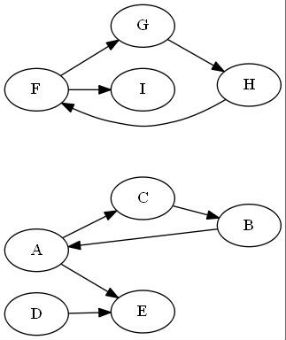
\includegraphics[scale=0.7,trim=3 3 3 3,clip]{2_2_0}
    \caption{L'image ci-dessus présente un graphe non connexe composé de deux sous graphes.}
\end{figure}

\begin{figure}[!h]
    \centering
    %\textbf{Your title}\par\medskip
    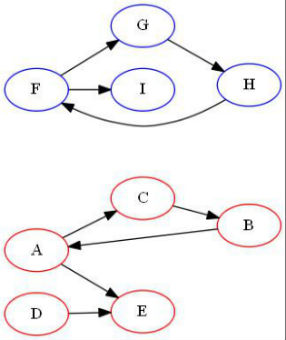
\includegraphics[scale=0.7,trim=3 3 3 3,clip]{2_2_1}
    \caption{Après exécution de l'algorithme, ces deux sous-graphes seront interprétés comme deux communautés distinctes.}
\end{figure}

\FloatBarrier
\section{Identification des hubs sociaux}
\subsection{Description}
L'identification des hubs sociaux d'une communauté consiste en l'identification des noeuds dont la suppression scinderait celle-ci en deux ou plusieurs communautés.

Une condition supplémentaire est que ce noeud doit diviser une communauté en communautés d'au moins $K$ éléments, où $K$ est donné comme paramètre à l'algorithme.

\subsection{Implémentation}

Un hub social correspond un point d'articulation d'un graphe. 
Ainsi, une recherche des points d'articulation du graphe représentant la communauté permet d'identifier les hubs sociaux de celle-ci.

Une fois tous les points d'articulation identifiés, il faut vérifier la condition supplémentaire afin de ne renvoyer que les points divisant le graphe en sous-graphes dont le nombre de noeuds est $>=K$.\\\\
Compléxité: $O(n+e)$ ou $n$ est le nombre de noeuds et $e$ est le nombre d'arcs.
\newpage
\subsubsection{Pseudocode}
\begin{algorithm}[H]
\Al{HubFinder}{
 \Fn{findallhubs}{
  \KwData{communitiesingraph}
   \For{each community in communitiesingraph}{
    \For{each node in community}{
     \If{node not visited}{
       explorehub(community, node)     
     }
   }
  }
 }
 \Fn{explorehub}{
  \KwData{community,current}
   \KwResult{List of hubs}
  timelist[current] = visitedtime\\
  lowesttime[current]=visitedtime\\
  visited[current]=True\\
  visitedtime++\\
  \For{each adjacent of current node}{
	 \If{adjacent not visited}{
	 	predecessor[adjacent] = current\\
	 	successors++\\
		call explorehub(adjacent)\\
		lowest time of current = min(lowest time of adjacent,\\
		\If{current is root and successors > 1 or !root and !backedge}{	
			\If{ current not in List of hubs}{
				add current to List of hubs}		
			}
		
	 }
	 \ElseIf{adjacent is not parent of current}{
		lowest child time=min(lowest child time, adjacent discovery time)	 	
	 	}
  }
  }
}
\end{algorithm}
\newpage
\FloatBarrier
\subsection{Exemple}

\begin{figure}[!h]
    \centering
    %\textbf{Your title}\par\medskip
    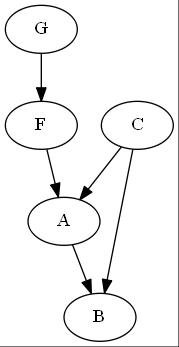
\includegraphics[scale=0.7,trim=3 3 3 3,clip]{2_3_0}
    \caption{Cette image montre un graphe connexe.}
\end{figure}

\begin{figure}[!h]
    \centering
    %\textbf{Your title}\par\medskip
    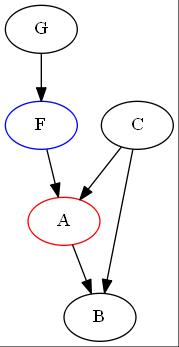
\includegraphics[scale=0.7,trim=3 3 3 3,clip]{2_3_1}
    \caption{Ce graphe présente les points d'articulation $A$ et $F$.}
\end{figure}

\begin{figure}[!h]
    \centering
    %\textbf{Your title}\par\medskip
    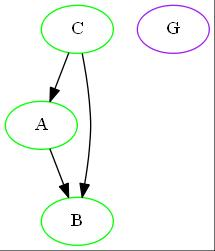
\includegraphics[scale=0.7,trim=3 3 3 3,clip]{APResult3_1}
    \caption{Le point $F$ divise le graphe en 2 communautés: {$CAB$} et {$G$} }
\end{figure}

\begin{figure}[!h]
    \centering
    %\textbf{Your title}\par\medskip
    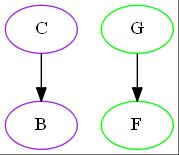
\includegraphics[scale=0.7,trim=3 3 3 3,clip]{APResult2_2}
    \caption{Le point $A$ divise le graphe en 2 communautés: {$CB$} et {$GF$} }
\end{figure}
\newpage
\FloatBarrier
\section{Travail en Equipe}
Repartition du travail:
\begin{itemize}
\item Simplification de dettes: Pavlo Polinetskyi
\item Identification des communautés: Grigore Antoniuc
\item Identification de Hubs Sociaux: Grigore Antoniuc
\item Refactorisation du code finale: Pavlo Polinetskyi
\item Ecriture des tests: Pavlo Polinetskyi
\item Rapport: Ensemble
\end{itemize}
\bigskip

Difficultés rencontrées:
\begin{itemize}
\item Synchronisation du code (Appréhension de Github)
\item Adaptation des algorithmes existants pour la resolution du problème posé
\item Ecriture d'un rapport complet en equipe en LaTeX
\end{itemize}
\section{Sources}
\begin{itemize}
\item Algorithme de Tarjan: Syllabus
\item Algorithme de Johnson: \url{http://people.cs.vt.edu/~gback/ICPCHandbook/book/copiesfromweb/circuits\_johnson.pdf}
\item Algorithme de Communauté (Parcours en profondeur): Syllabus
\item Algorithme de Hubs Sociaux (Point d'articulation): Syllabus
\end{itemize}

\section{Tests}
\subsection{OurTests.py}
Fichier à executer pour lancer les tests prédéfinis par nous pour chaque algorithme.\\
Voici les representations graphiques des graphes utilisés:
\subsubsection{Tests de simplification de dettes}
Test 1:
\begin{figure}[!h]
    \centering
    %\textbf{Your title}\par\medskip
    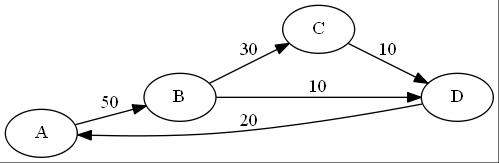
\includegraphics[scale=0.7,trim=3 3 3 3,clip]{simplify1before}
    \caption{Avant Simplification}
\end{figure}
\begin{figure}[!h]
    \centering
    %\textbf{Your title}\par\medskip
    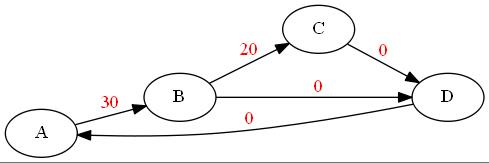
\includegraphics[scale=0.7,trim=3 3 3 3,clip]{simplify1after}
    \caption{Après Simplification}
\end{figure}
\newpage
\FloatBarrier
Test 2:
\begin{figure}[!h]
    \centering
    %\textbf{Your title}\par\medskip
    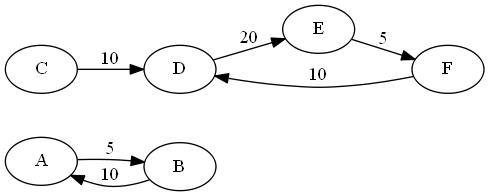
\includegraphics[scale=0.7,trim=3 3 3 3,clip]{simplify2before}
    \caption{Avant Simplification}
\end{figure}
\begin{figure}[!h]
    \centering
    %\textbf{Your title}\par\medskip
    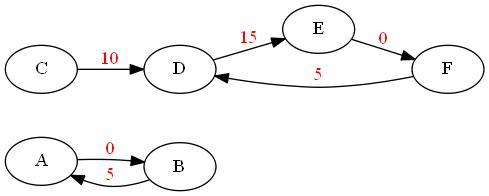
\includegraphics[scale=0.7,trim=3 3 3 3,clip]{simplify2after}
    \caption{Après Simplification}
\end{figure}
\newpage
\FloatBarrier
\subsubsection{Test d'identification de communautés}
Test 1:
\begin{figure}[!h]
    \centering
    %\textbf{Your title}\par\medskip
    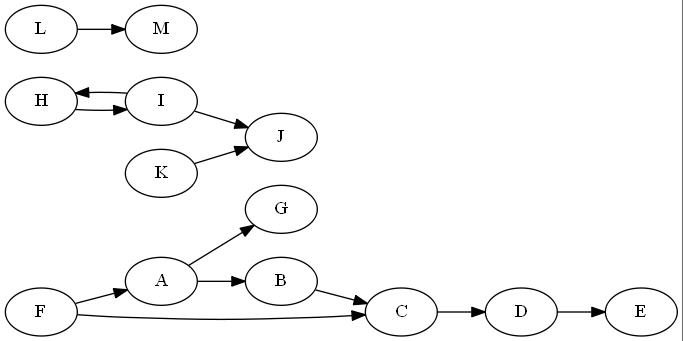
\includegraphics[scale=0.7,trim=3 3 3 3,clip]{community1}
    \caption{Résultat attendu: [[G, A, B, C, D, E, F], [I, H, J, K], [M, L]]}
\end{figure}
\newpage
\FloatBarrier
\subsubsection{Test d'identification de Hubs Sociaux}
Test 1:\\
\begin{figure}[!h]
    \centering
    %\textbf{Your title}\par\medskip
    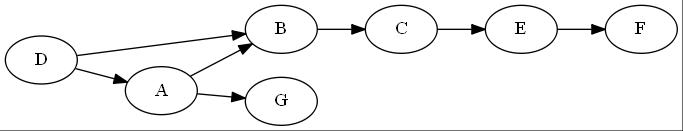
\includegraphics[scale=0.7,trim=3 3 3 3,clip]{artipointdefault}
    \caption{Le graphe}
\end{figure}
\begin{figure}[!h]
    \centering
    %\textbf{Your title}\par\medskip
    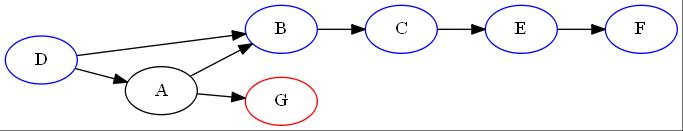
\includegraphics[scale=0.7,trim=3 3 3 3,clip]{artipointA}
    \caption{Division en le point A}
\end{figure}
\begin{figure}[!h]
    \centering
    %\textbf{Your title}\par\medskip
    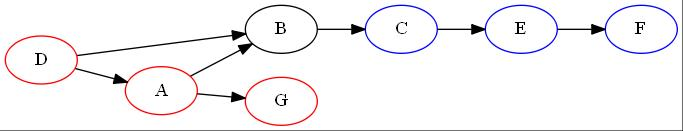
\includegraphics[scale=0.7,trim=3 3 3 3,clip]{artipointB}
    \caption{Division en le point B}
\end{figure}
\begin{figure}[!h]
    \centering
    %\textbf{Your title}\par\medskip
    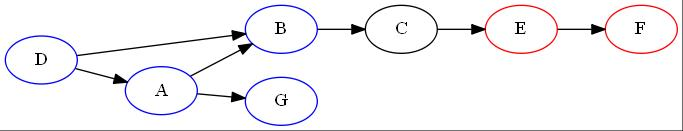
\includegraphics[scale=0.7,trim=3 3 3 3,clip]{artipointC}
    \caption{Division en le point C}
\end{figure}
\begin{figure}[!h]
    \centering
    %\textbf{Your title}\par\medskip
    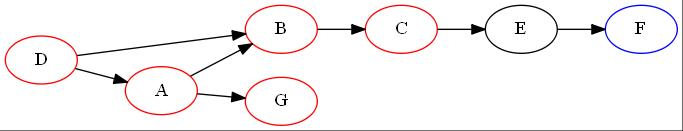
\includegraphics[scale=0.7,trim=3 3 3 3,clip]{artipointE}
    \caption{Division en le point E}
\end{figure}
\FloatBarrier
Alors les résultats attendus sont:
\begin{itemize}
\item Pour K=1: [E, C, A, B]
\item Pour K=2: [C, B]
\item Pour K=3: [B]
\item Pour K=4: []
\end{itemize}

\subsection{YourTester.py}
Afin de tester les algorithmes avec vos propres tests, lancez le fichier YourTester.py. Voici un exemple d'utilisation:\\
\textbf{\textit{python3 YourTester.py inputfile.txt -a -k 9}}\\\\
YourTester.py utilise la librarie argparse, alors pour afficher plus d'infomations il suffit juste de taper:\\
\textbf{\textit{python3 YourTester.py -h}}\\\\
Voici la liste des arguments possibles:
\begin{itemize}
\item -k chiffre
\item --simplify 
\item --communities
\item --hubs
\item -a --all
\end{itemize}
\end{document}

